% Options for packages loaded elsewhere
\PassOptionsToPackage{unicode}{hyperref}
\PassOptionsToPackage{hyphens}{url}
\PassOptionsToPackage{dvipsnames,svgnames,x11names}{xcolor}
%
\documentclass[
  letterpaper,
  DIV=11,
  numbers=noendperiod]{scrreprt}

\usepackage{amsmath,amssymb}
\usepackage{iftex}
\ifPDFTeX
  \usepackage[T1]{fontenc}
  \usepackage[utf8]{inputenc}
  \usepackage{textcomp} % provide euro and other symbols
\else % if luatex or xetex
  \usepackage{unicode-math}
  \defaultfontfeatures{Scale=MatchLowercase}
  \defaultfontfeatures[\rmfamily]{Ligatures=TeX,Scale=1}
\fi
\usepackage{lmodern}
\ifPDFTeX\else  
    % xetex/luatex font selection
\fi
% Use upquote if available, for straight quotes in verbatim environments
\IfFileExists{upquote.sty}{\usepackage{upquote}}{}
\IfFileExists{microtype.sty}{% use microtype if available
  \usepackage[]{microtype}
  \UseMicrotypeSet[protrusion]{basicmath} % disable protrusion for tt fonts
}{}
\makeatletter
\@ifundefined{KOMAClassName}{% if non-KOMA class
  \IfFileExists{parskip.sty}{%
    \usepackage{parskip}
  }{% else
    \setlength{\parindent}{0pt}
    \setlength{\parskip}{6pt plus 2pt minus 1pt}}
}{% if KOMA class
  \KOMAoptions{parskip=half}}
\makeatother
\usepackage{xcolor}
\setlength{\emergencystretch}{3em} % prevent overfull lines
\setcounter{secnumdepth}{5}
% Make \paragraph and \subparagraph free-standing
\makeatletter
\ifx\paragraph\undefined\else
  \let\oldparagraph\paragraph
  \renewcommand{\paragraph}{
    \@ifstar
      \xxxParagraphStar
      \xxxParagraphNoStar
  }
  \newcommand{\xxxParagraphStar}[1]{\oldparagraph*{#1}\mbox{}}
  \newcommand{\xxxParagraphNoStar}[1]{\oldparagraph{#1}\mbox{}}
\fi
\ifx\subparagraph\undefined\else
  \let\oldsubparagraph\subparagraph
  \renewcommand{\subparagraph}{
    \@ifstar
      \xxxSubParagraphStar
      \xxxSubParagraphNoStar
  }
  \newcommand{\xxxSubParagraphStar}[1]{\oldsubparagraph*{#1}\mbox{}}
  \newcommand{\xxxSubParagraphNoStar}[1]{\oldsubparagraph{#1}\mbox{}}
\fi
\makeatother


\providecommand{\tightlist}{%
  \setlength{\itemsep}{0pt}\setlength{\parskip}{0pt}}\usepackage{longtable,booktabs,array}
\usepackage{calc} % for calculating minipage widths
% Correct order of tables after \paragraph or \subparagraph
\usepackage{etoolbox}
\makeatletter
\patchcmd\longtable{\par}{\if@noskipsec\mbox{}\fi\par}{}{}
\makeatother
% Allow footnotes in longtable head/foot
\IfFileExists{footnotehyper.sty}{\usepackage{footnotehyper}}{\usepackage{footnote}}
\makesavenoteenv{longtable}
\usepackage{graphicx}
\makeatletter
\def\maxwidth{\ifdim\Gin@nat@width>\linewidth\linewidth\else\Gin@nat@width\fi}
\def\maxheight{\ifdim\Gin@nat@height>\textheight\textheight\else\Gin@nat@height\fi}
\makeatother
% Scale images if necessary, so that they will not overflow the page
% margins by default, and it is still possible to overwrite the defaults
% using explicit options in \includegraphics[width, height, ...]{}
\setkeys{Gin}{width=\maxwidth,height=\maxheight,keepaspectratio}
% Set default figure placement to htbp
\makeatletter
\def\fps@figure{htbp}
\makeatother

\KOMAoption{captions}{tableheading}
\makeatletter
\@ifpackageloaded{bookmark}{}{\usepackage{bookmark}}
\makeatother
\makeatletter
\@ifpackageloaded{caption}{}{\usepackage{caption}}
\AtBeginDocument{%
\ifdefined\contentsname
  \renewcommand*\contentsname{Table of contents}
\else
  \newcommand\contentsname{Table of contents}
\fi
\ifdefined\listfigurename
  \renewcommand*\listfigurename{List of Figures}
\else
  \newcommand\listfigurename{List of Figures}
\fi
\ifdefined\listtablename
  \renewcommand*\listtablename{List of Tables}
\else
  \newcommand\listtablename{List of Tables}
\fi
\ifdefined\figurename
  \renewcommand*\figurename{Figure}
\else
  \newcommand\figurename{Figure}
\fi
\ifdefined\tablename
  \renewcommand*\tablename{Table}
\else
  \newcommand\tablename{Table}
\fi
}
\@ifpackageloaded{float}{}{\usepackage{float}}
\floatstyle{ruled}
\@ifundefined{c@chapter}{\newfloat{codelisting}{h}{lop}}{\newfloat{codelisting}{h}{lop}[chapter]}
\floatname{codelisting}{Listing}
\newcommand*\listoflistings{\listof{codelisting}{List of Listings}}
\makeatother
\makeatletter
\makeatother
\makeatletter
\@ifpackageloaded{caption}{}{\usepackage{caption}}
\@ifpackageloaded{subcaption}{}{\usepackage{subcaption}}
\makeatother

\ifLuaTeX
  \usepackage{selnolig}  % disable illegal ligatures
\fi
\usepackage{bookmark}

\IfFileExists{xurl.sty}{\usepackage{xurl}}{} % add URL line breaks if available
\urlstyle{same} % disable monospaced font for URLs
\hypersetup{
  pdftitle={Workshop Handbook},
  pdfauthor={Neha Moopen \& Lilli van Wielink},
  colorlinks=true,
  linkcolor={blue},
  filecolor={Maroon},
  citecolor={Blue},
  urlcolor={Blue},
  pdfcreator={LaTeX via pandoc}}


\title{Workshop Handbook}
\author{Neha Moopen \& Lilli van Wielink}
\date{2024-08-12}

\begin{document}
\maketitle

\renewcommand*\contentsname{Table of contents}
{
\hypersetup{linkcolor=}
\setcounter{tocdepth}{2}
\tableofcontents
}

\bookmarksetup{startatroot}

\chapter*{Welcome}\label{welcome}
\addcontentsline{toc}{chapter}{Welcome}

\markboth{Welcome}{Welcome}

The UB \& ITS collaborate on workshops aimed at working with data and
software in line with Open Science and FAIR Principles. As our
collaboration grows closer within and between workshops, this Handbook
is being developed as a common reference that consolidates information
on how we develop and organize these workshops.

\part{WORKSHOPS}

\section*{Ongoing Workshops}\label{ongoing-workshops}
\addcontentsline{toc}{section}{Ongoing Workshops}

\markright{Ongoing Workshops}

As of Academic Year 2023-2024, we are providing 7 \emph{standard}
workshops/e-learnings.

\subsection*{Research Data}\label{research-data}
\addcontentsline{toc}{subsection}{Research Data}

\begin{enumerate}
\def\labelenumi{\arabic{enumi}.}
\item
  Quickstart to Research Data Management
\item
  Getting Started With Yoda
\item
  Getting Started With Virtual Research Environments
\end{enumerate}

\subsection*{Research Software}\label{research-software}
\addcontentsline{toc}{subsection}{Research Software}

\begin{enumerate}
\def\labelenumi{\arabic{enumi}.}
\item
  Introduction to R \& Data:
  \href{https://utrechtuniversity.github.io/workshop-introduction-to-R-and-data/}{course
  website} /
  \href{https://github.com/UtrechtUniversity/workshop-introduction-to-r-and-data}{GitHub
  repository}
\item
  Introduction to Python:
\item
  Writing Reproducible Manuscripts in R \& Python:
  \href{https://nehamoopen.github.io/worcshop-book/}{course website} /
  \href{https://github.com/nehamoopen/worcshop-book}{GitHub repository}
\item
  Best Practices in Writing Reproducible Code:
  \href{https://utrechtuniversity.github.io/workshop-computational-reproducibility/docs/index.html}{course
  website} /
  \href{https://github.com/UtrechtUniversity/workshop-computational-reproducibility}{GitHub
  repository}
\end{enumerate}

\chapter*{Before}\label{before}
\addcontentsline{toc}{chapter}{Before}

\markboth{Before}{Before}

This section provides an overview of what needs to occur while planning
workshops for the upcoming academic year.

\section*{Jaarplanning}\label{jaarplanning}
\addcontentsline{toc}{section}{Jaarplanning}

\markright{Jaarplanning}

Before commencing with the jaarplanning, the department should decide on
which workshops will be offered (or not) and who will be involved in the
workshop as leads and instructors/helpers. This would likely be decided
during the Annual Review.

\subsection*{Workshop Agenda}\label{workshop-agenda}
\addcontentsline{toc}{subsection}{Workshop Agenda}

By the end of May, we should have the jaarplanning for the next academic
year ready.

When doing this jaarplanning, we should take the following into account:

\begin{itemize}
\tightlist
\item
  the \emph{frequency} of the workshop,
\item
  the \emph{preferred days} for the workshop,
\item
  the \emph{number of participants} for the workshop,
\end{itemize}

Moreover, the workshops should be \emph{spaced out} well, so we don't
have weeks that are too busy or vice versa.

Here is an example of the workshop agenda for 2023-2024:
\href{https://solisservices.sharepoint.com/:x:/r/sites/RDMSpeeltuin/Shared\%20Documents/General/Trainings\%20and\%20Workshops/Workshop\%20Communication\%20Materials/workshops-planning-2023-2024.xlsx?d=w0037faec227d49c09d11be856d3c3cbb&csf=1&web=1&e=06E4BJ&nav=MTVfezAwMDAwMDAwLTAwMDEtMDAwMC0wMDAwLTAwMDAwMDAwMDAwMH0}{RDM
Support -\textgreater{} General -\textgreater{} Training \& Workshops
-\textgreater{} Workshop Communication Materials -\textgreater{}
workshops-planning-2023-2024.xlsx}

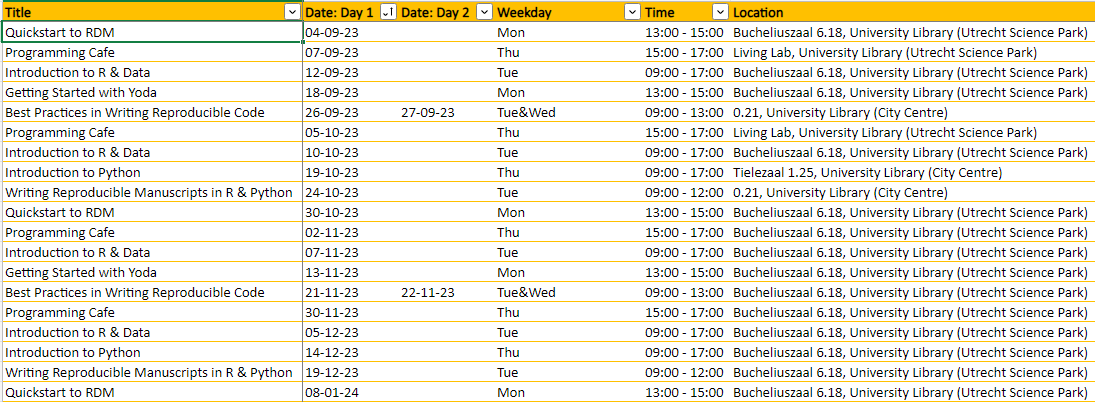
\includegraphics{images/workshop-agenda.PNG}

\subsection*{Room Booking}\label{room-booking}
\addcontentsline{toc}{subsection}{Room Booking}

We need to book locations for all the workshops in advance. This can be
done via the the booking system or by contacting colleagues in
\emph{Publieksdiensten} (probably not called the same now after the
reorganization).

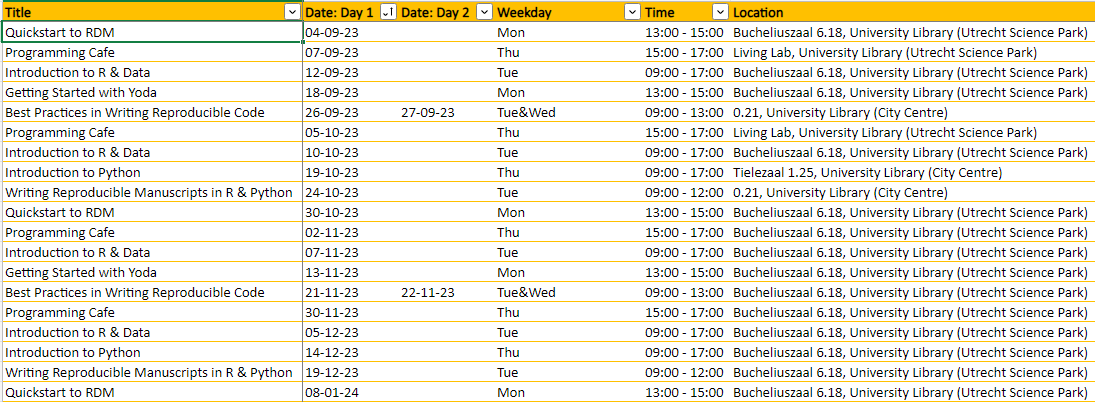
\includegraphics{images/workshop-agenda.PNG}

\subsection*{Outlook Calendar}\label{outlook-calendar}
\addcontentsline{toc}{subsection}{Outlook Calendar}

When the jaarplanning is done, put it in an Outlook calendar that can be
shared with everyone.

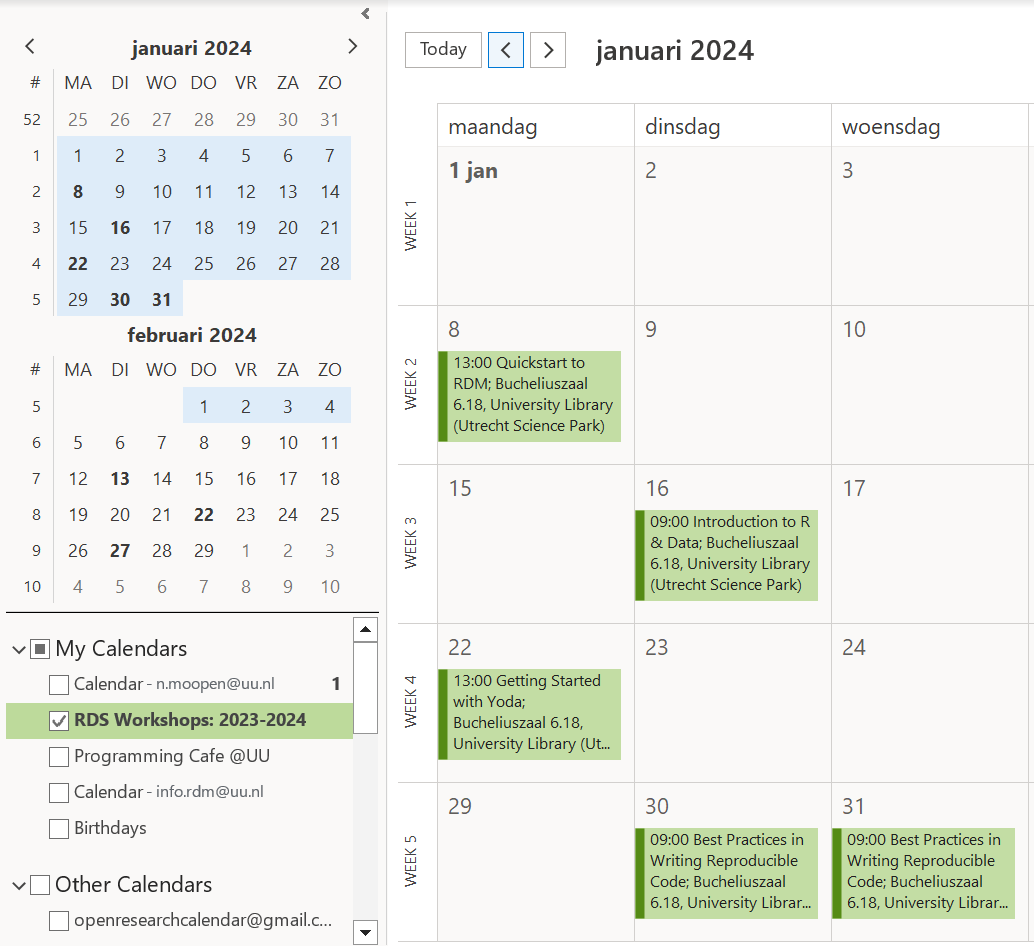
\includegraphics{images/outlook-calendar.PNG}

You can use the Excel sheet from the jaarplanning to create calendar
items in bulk. Here are two links for reference:

\begin{enumerate}
\def\labelenumi{\arabic{enumi}.}
\item
  \href{https://www.techrepublic.com/article/how-to-import-excel-records-into-an-outlook-calendar/}{example
  1}
\item
  \href{https://www.auditexcel.co.za/blog/import-excel-appointments-into-outlook-calendar/}{example
  2}
\end{enumerate}

After that, you can choose to either share or publish your Outlook
calendar:

\begin{itemize}
\tightlist
\item
  https://support.microsoft.com/en-us/office/share-your-calendar-in-outlook-com-0fc1cb48-569d-4d1e-ac20-5a9b3f5e6ff2
\end{itemize}

\subsection*{Sign Up Sheet}\label{sign-up-sheet}
\addcontentsline{toc}{subsection}{Sign Up Sheet}

Also make a page where people can sign up or simply report who will be
going.

May be redundant with the pool of instructors and helpers but might
still help maintain overview. Maybe sign up for the whole academic year
/ commit to one workshop and then figure it out within your team. To be
discussed.

Here is a link to the sign-up sheet for 2023-2024:
\href{https://teams.microsoft.com/l/entity/26bc2873-6023-480c-a11b-76b66605ce8c/_djb2_msteams_prefix_1765026388?context=\%7B\%22channelId\%22\%3A\%2219\%3Aa5f3eb9fa731402c91171d0ef1eed535\%40thread.skype\%22\%7D&tenantId=d72758a0-a446-4e0f-a0aa-4bf95a4a10e7}{RDM
Support -\textgreater{} Team Code and Software -\textgreater{} Workshops
\& Cafes (tab)}

The Excel sheet can also be used as a basis for creating this sign-up
sheet tab, you don't have to create entries separately.

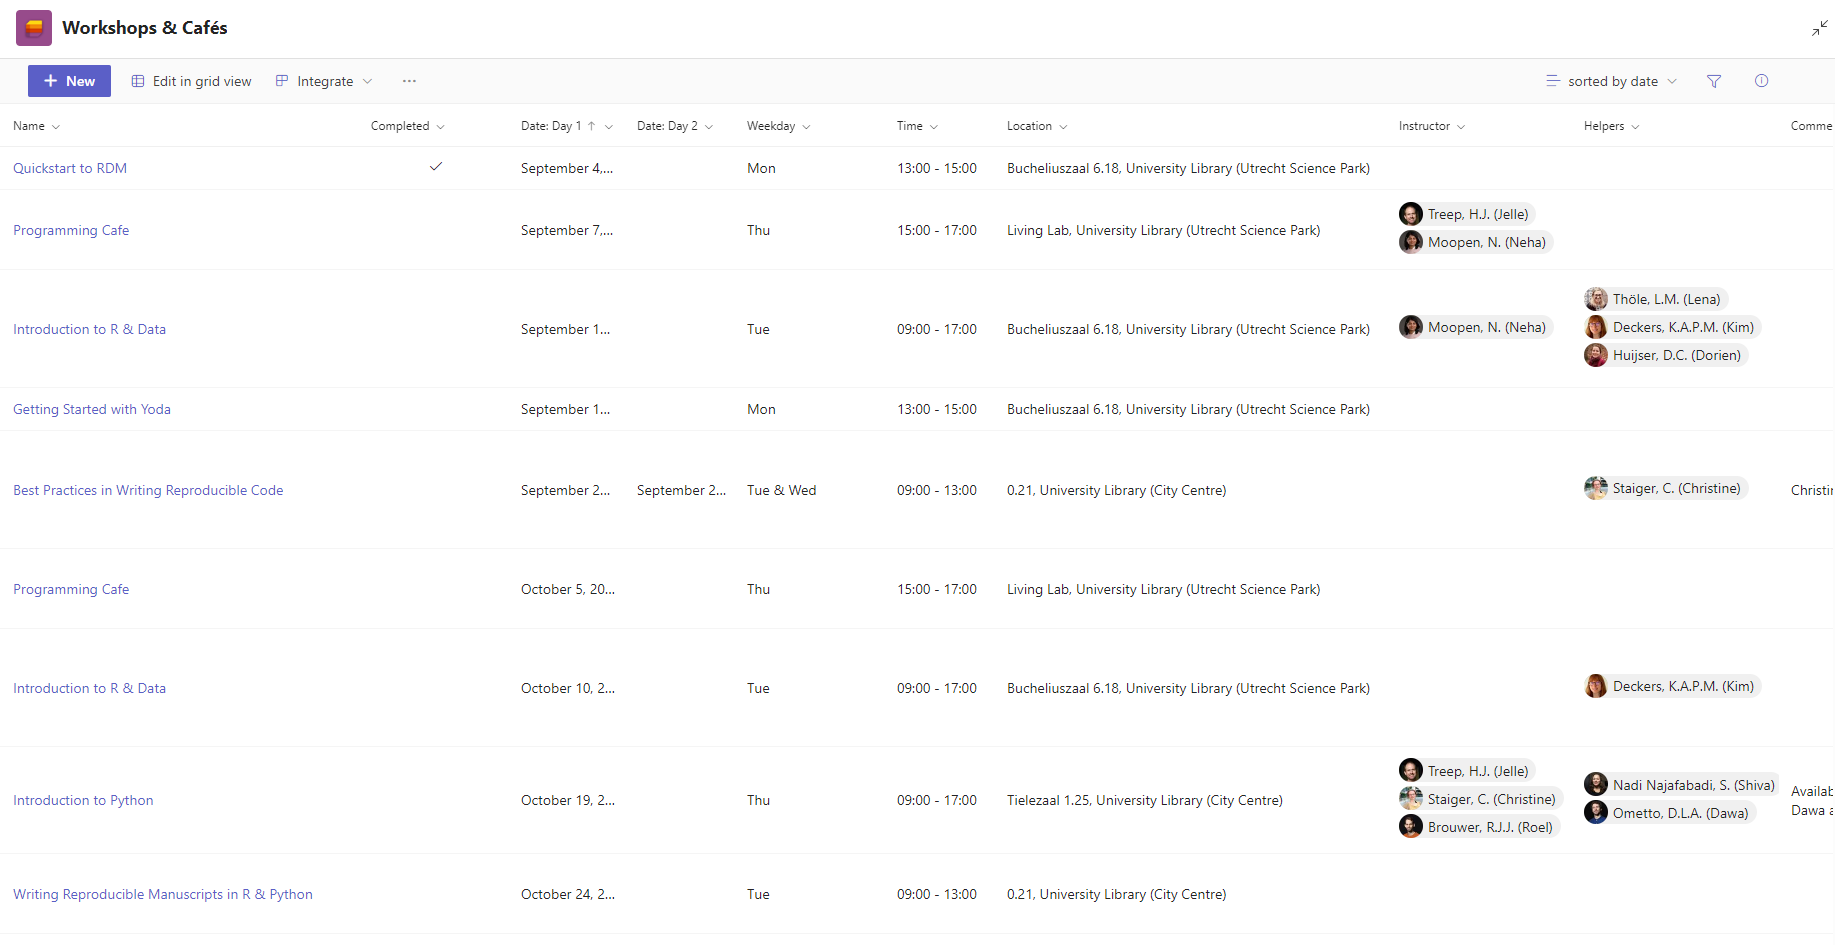
\includegraphics{images/sign-up-sheet.PNG}

\section*{Website}\label{website}
\addcontentsline{toc}{section}{Website}

\markright{Website}

The following folder contains (per workshop) all the texts for landing
pages, agenda items, Formdesk forms and confirmations, pre- and
post-workshop emails:
\href{https://solisservices.sharepoint.com/:f:/r/sites/RDMSpeeltuin/Shared\%20Documents/General/Trainings\%20and\%20Workshops/Workshop\%20Communication\%20Materials?csf=1&web=1&e=dab1La}{RDM
Support -\textgreater{} General -\textgreater{} Training \& Workshops
-\textgreater{} Workshop Communication Materials}

There is also an Excel sheet to track the review and update of
materials:
\href{https://solisservices.sharepoint.com/:x:/r/sites/RDMSpeeltuin/Shared\%20Documents/General/Trainings\%20and\%20Workshops/Workshop\%20Communication\%20Materials/workshops-planning-2023-2024.xlsx?d=w0037faec227d49c09d11be856d3c3cbb&csf=1&web=1&e=ggINu4&nav=MTVfezYzREREOTdELTNBNkMtNDJDOS1BRTQ2LTFDNzQ2MzBFMzZBRX0}{}

\begin{figure}[H]

{\centering 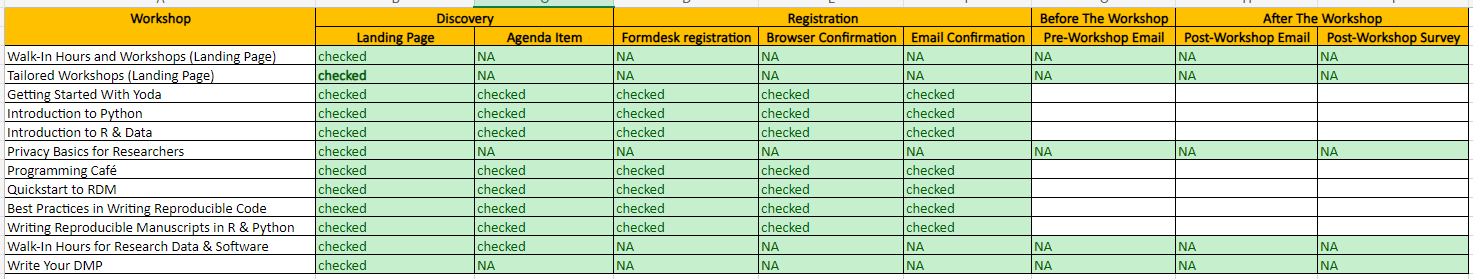
\includegraphics{images/workshop-materials-checklist.PNG}

}

\caption{RDM Support -\textgreater{} General -\textgreater{} Training \&
Workshops -\textgreater{} Workshop Communication Materials
-\textgreater{} workshops-planning-2023-2024.xlsx}

\end{figure}%

\subsection*{Landing Page}\label{landing-page}
\addcontentsline{toc}{subsection}{Landing Page}

Review the landing page text for all workshops. Lilli makes template and
the workshop leads do the reviewing (primarily of workshop
description/content, the more admin stuff will be generic).

Example of landing page for Introduction to R \& Data:
\url{https://www.uu.nl/en/research/research-data-management/training-workshops/introduction-to-r-data}

The landing page is a generic description of the workshop and includes
an overview of all workshop dates with link to the specific agenda item.

\begin{itemize}
\tightlist
\item
  prerequisties
\item
  what you can expect (or not)
\item
  UU and UU-affiliated only
\item
  costs
\item
  deregistration and no-show/dropout policy
\end{itemize}

Note that a Dutch translation will be needed as well.

\subsection*{Agenda Items}\label{agenda-items}
\addcontentsline{toc}{subsection}{Agenda Items}

The agenda item is specific to a workshop date/occurence and includes
the link to the registration form.

Example of agenda item for Introduction to R \& Data:
\url{https://www.uu.nl/en/events/introduction-to-r-data-may-2024}

Note that a Dutch translation will be needed as well.

\section*{Formdesk}\label{formdesk}
\addcontentsline{toc}{section}{Formdesk}

\markright{Formdesk}

How to handle waitlists? Maximum number of participants? Maximum number
of waitlisted participants?

\subsection*{Formdesk Form}\label{formdesk-form}
\addcontentsline{toc}{subsection}{Formdesk Form}

The Formdesk registration form is largely the same for all workshops.
There are generic questions related to registration, but a couple of
specific questions per workshop.

Make sure that the werkstudenten ensure only UU and UU-affiliated
addresses are accepted for registration! Provide a list of these
addresses (UMCU, PMC, etc.)

Here is a link to the default questions for Formdesk at the moment:
\href{https://solisservices.sharepoint.com/:w:/r/sites/RDMSpeeltuin/Shared\%20Documents/General/Trainings\%20and\%20Workshops/Workshop\%20Communication\%20Materials/_formdesk/default-questions-formdesk-registration.docx?d=wdc1e2777ebe8453bb61f453f106e50fc&csf=1&web=1&e=Vxd94A}{RDM
Support -\textgreater{} General -\textgreater{} Training \& Workshops
-\textgreater{} Workshop Communication Materials -\textgreater{}
\_formdesk -\textgreater{} default-questions-formdesk-registration.docx}

\subsection*{Browser Confirmation}\label{browser-confirmation}
\addcontentsline{toc}{subsection}{Browser Confirmation}

This refers to the text that appears in your browser when the
registration is confirmed. It points to \url{info.rdm@uu.nl} as contact
point in case a confirmation email is not received.

\href{https://solisservices.sharepoint.com/:w:/r/sites/RDMSpeeltuin/Shared\%20Documents/General/Trainings\%20and\%20Workshops/Workshop\%20Communication\%20Materials/_formdesk/default-formdesk-confirmation.docx?d=wee2a03a810e74d40aeea4e8cb1e5be6b&csf=1&web=1&e=PBbgGp}{RDM
Support -\textgreater{} General -\textgreater{} Training \& Workshops
-\textgreater{} Workshop Communication Materials -\textgreater{}
\_formdesk -\textgreater{} default-questions-formdesk-confirmation.docx}

\subsection*{Confirmation Email}\label{confirmation-email}
\addcontentsline{toc}{subsection}{Confirmation Email}

This refers to the email that participants receive when their
registration is confirmed. It points to \url{info.rdm@uu.nl} as contact
point and includes a personalized link for deregistration.

\href{https://solisservices.sharepoint.com/:w:/r/sites/RDMSpeeltuin/Shared\%20Documents/General/Trainings\%20and\%20Workshops/Workshop\%20Communication\%20Materials/_formdesk/default-formdesk-confirmation.docx?d=wee2a03a810e74d40aeea4e8cb1e5be6b&csf=1&web=1&e=PBbgGp}{RDM
Support -\textgreater{} General -\textgreater{} Training \& Workshops
-\textgreater{} Workshop Communication Materials -\textgreater{}
\_formdesk -\textgreater{} default-questions-formdesk-confirmation.docx}

We might want to consider putting the pre-workshop email in the Formdesk
confirmation email already?

\section*{Werkstudenten}\label{werkstudenten}
\addcontentsline{toc}{section}{Werkstudenten}

\markright{Werkstudenten}

Once all the documents have been reviewed and/or updated, have the
Communicatie werkstudenten put everything online. They can be contacted
at: werkstudentCC@uu.nl

It can take them up to a month to process everything for a whole
academic year. We naturally want to prioritize the workshops from
September-December, so people can already start signing up for that.

Some things they should do: number of participants, UU \& UU-affiliated
addresses, specify the owners and co-owners for the form, notification
if it's registration less than 7 days.

It would be helpful to give them a briefing of instructions like in this
document:
\href{https://solisservices.sharepoint.com/:w:/r/sites/RDMSpeeltuin/Shared\%20Documents/General/Trainings\%20and\%20Workshops/Workshop\%20Communication\%20Materials/briefing-work-students\%20.docx?d=wd1d0b1b5d61e432699f668dfe89ae60f&csf=1&web=1&e=iVl4Iz}{RDM
Support -\textgreater{} General -\textgreater{} Training \& Workshops
-\textgreater{} Workshop Communication Materials -\textgreater{}
briefing-work-students.docx}

\subsection*{New}\label{new}
\addcontentsline{toc}{subsection}{New}

\begin{itemize}
\tightlist
\item
  We need a TIMELINE for the jaarplanning and coordination -- when do we
  wanna schedule big group meetings, review moments, determine leads 🎉
\item
  Create a TASK BOARD for workshops if we think it's useful.
\item
  List the workshops + e-learnings we want do/maintain next academic
  year. Determine what to do with stuff that might be phased out (if at
  all). You might archive it for example.
\item
  Determine the leads of these workshops, as well as a pool of
  instructors and helpers per workshop. Clarify and agree on what these
  roles mean and involve (and not).
\end{itemize}

\chapter*{During}\label{during}
\addcontentsline{toc}{chapter}{During}

\markboth{During}{During}

This section provides an overview of what needs to occur during the
academic year as we go through the planned workshops.

\section*{Communication}\label{communication}
\addcontentsline{toc}{section}{Communication}

\markright{Communication}

\subsection*{Q\&A}\label{qa}
\addcontentsline{toc}{subsection}{Q\&A}

Any Q\&A or communication about the workshops should go through TopDesk.
The workshop leads are responsible for picking up calls related to their
respective workshops. Any other calls can be picked by the workshop
coordinator or the team member monitoring TopDesk that day, depending on
what is required.

\subsection*{Waitlists}\label{waitlists}
\addcontentsline{toc}{subsection}{Waitlists}

Currently, requests to be waitlisted for workshops are directed to
TopDesk. The workshop lead should:

\begin{itemize}
\tightlist
\item
  place the call under their name
\item
  set the due date to one week before the workshop
\item
  send a response acknowledging the waitlist request (TODO: make a
  template)
\end{itemize}

\section*{Pre-Workshop}\label{pre-workshop}
\addcontentsline{toc}{section}{Pre-Workshop}

\markright{Pre-Workshop}

\subsection*{Pre-Workshop Email}\label{pre-workshop-email}
\addcontentsline{toc}{subsection}{Pre-Workshop Email}

The pre-workshop email should be sent out \emph{one week} before the
workshop is to take place. The email should be placed within an Outlook
appointment. The workshop lead has primary responsibility for this.

The following folder contains (per workshop) all the texts for pre- and
post-workshop emails:
\href{https://solisservices.sharepoint.com/:f:/r/sites/RDMSpeeltuin/Shared\%20Documents/General/Trainings\%20and\%20Workshops/Workshop\%20Communication\%20Materials?csf=1&web=1&e=dab1La}{RDM
Support -\textgreater{} General -\textgreater{} Training \& Workshops
-\textgreater{} Workshop Communication Materials}

TODO: review pre-workshop email in general, but also include
deregistration reminder and no-show/dropout policy.

\subsection*{Catering}\label{catering}
\addcontentsline{toc}{subsection}{Catering}

We are currently arranging tea and coffee ourselves. If a budget for
catering is arranged, the workshop lead will need to book the catering
at least \textgreater=3 days before the workshop is to take place.

\section*{Workshop}\label{workshop}
\addcontentsline{toc}{section}{Workshop}

\markright{Workshop}

During the workshop, we distinguish between \emph{Instructors} and
\emph{Helpers} in terms of our role for that day. The \emph{Instructor}
is responsible for teaching: they are at the front of the room and go
through the slides and demos. The \emph{Helper} is responsible for
walking around the room and supporting participants during the workshop,
especially during the exercises. These are not fixed roles, we expect
colleagues will take turns with a different role every time a workshop
takes place. For those who are new to the workshop, it may be helpful to
be a \emph{Helper} for a couple of rounds before picking up the
\emph{Instructor} role.

It's helpful if at least 2 colleagues arrive earlier to open the room
and help set up the space.

We also want to take attendance during the workshop to keep our numbers
up to date: \emph{registrants}, \emph{deregistrants}, \emph{attendees},
\emph{no-shows}.

Start the workshop with a round of introductions. End the workshop with
necessary closing information.

After the workshop, it may be helpful to have an informal discussion on
how the workshop went. Feedback can be exchanged and questions can be
answered. If there are action points, the workshop lead can pick them up
or make GitHub Issues if needed.

\section*{Post-Workshop}\label{post-workshop}
\addcontentsline{toc}{section}{Post-Workshop}

\markright{Post-Workshop}

\subsection*{Post-Workshop Email}\label{post-workshop-email}
\addcontentsline{toc}{subsection}{Post-Workshop Email}

The post-workshop email should be sent out as soon as possible after the
workshop, ideally the very next day but not later than 1 week after the
workshop. The workshop lead has primary responsibility for this.

The following folder contains (per workshop) all the texts for pre- and
post-workshop emails:
\href{https://solisservices.sharepoint.com/:f:/r/sites/RDMSpeeltuin/Shared\%20Documents/General/Trainings\%20and\%20Workshops/Workshop\%20Communication\%20Materials?csf=1&web=1&e=dab1La}{RDM
Support -\textgreater{} General -\textgreater{} Training \& Workshops
-\textgreater{} Workshop Communication Materials}

TODO: The workshop lead should update the Excel sheet tracking
workshop-related numbers, i.e.~\emph{registrants}, \emph{deregistrants},
\emph{attendees}, \emph{no-shows}.

\section*{Quarterly Review}\label{quarterly-review}
\addcontentsline{toc}{section}{Quarterly Review}

\markright{Quarterly Review}

\subsection*{Pizza Party}\label{pizza-party}
\addcontentsline{toc}{subsection}{Pizza Party}

The workshop coordinator will organize a Quarterly Review, hopefully
with pizza to discuss how things are going.

\subsection*{Post-Workshop Survey}\label{post-workshop-survey}
\addcontentsline{toc}{subsection}{Post-Workshop Survey}

The post-workshop email contains a link to the post-workshop survey. The
survey is hosted on Qualtrics and a report can be derived on a quarterly
and annual basis to evaluate workshop-related feedback from
participants.

\chapter*{After}\label{after}
\addcontentsline{toc}{chapter}{After}

\markboth{After}{After}

This section provides an overview of what needs to occur towards the end
of the academic year, as we get closer to wrapping up all the workshops.

The `timing' of activities in this section will overlap with those
associated with planning for the upcoming academic year, but they serve
different purposes.

\section*{Annual Review}\label{annual-review}
\addcontentsline{toc}{section}{Annual Review}

\markright{Annual Review}

During the Annual Review, we reflect on the year as a whole and what we
might want to do differently in the upcoming year. In addition to
evaluating the pre- and post-workshop surveys and our experiences in
general. The following decisions can be made:

\begin{itemize}
\tightlist
\item
  which workshops will be provided the next year
\item
  who will comprise the sub-team for each workshop
\item
  who will be the workshop lead
\item
  what are the action points and to-dos that need to be carried our as
  part of the jaarplanning
\item
  what is the planning/timeline towards implementing the action points
\item
  what is needed from everyone to develop themselves and have a good
  time teaching the workshops
\end{itemize}

\section*{Workshop Materials}\label{workshop-materials}
\addcontentsline{toc}{section}{Workshop Materials}

\markright{Workshop Materials}

\subsection*{Maintenance}\label{maintenance}
\addcontentsline{toc}{subsection}{Maintenance}

After the last workshop has taken place, all associated materials should
be archived on Zenodo.

\begin{itemize}
\item
  Workshops related to \emph{data} are typically PowerPoint
  presentations. These should be uploaded to Zenodo, along with a pdf
  copy.
\item
  Workshops related to \emph{software} have materials built with Quarto
  and hosted on the Utrecht University GitHub organization. The
  repositories on GitHub should be integrated with Zenodo first and a
  `release' of the repository should be made on an annual basis. Zenodo
  will detect the release and automatically archive it.
\end{itemize}

\subsection*{Development}\label{development}
\addcontentsline{toc}{subsection}{Development}

Teams for each workshop are encouraged to get together and work on
updating / developing the materials further. If colleagues switch
between workshops to one that the are not familiar with or if we have
new colleagues, this can be opportunity to get started with the workshop
`onboarding' process until the first workshop actually takes place.

\bookmarksetup{startatroot}

\chapter*{Custom Workshops}\label{custom-workshops}
\addcontentsline{toc}{chapter}{Custom Workshops}

\markboth{Custom Workshops}{Custom Workshops}

\begin{itemize}
\item
  We currently have a small paragraph for custom workshops at:
  \url{https://www.uu.nl/en/research/research-data-management/workshops}
\item
  TODO: a separate landing page for the custom workshops with a
  gallery/portfolio (links to Zenodo or GitHub) showing examples of
  custom workshops we have done?
\item
  Requests for custom workshops should be directed to the workshop
  coordinator via TopDesk.
\item
  The workshop coordinator will bring the request to the team and we
  will decide if we can do it and who will do it.
\item
  If the workshop can be carried out, the workshop coordinator will link
  the contactperson with the colleagues who are picking it up. They will
  also check with the contactperson about how they found out about us
  and our offering.
\item
  If possible, the post-workshop survey should be distributed to the
  attendees.
\item
  After the workshop, the colleagues will report back to the workshop
  coordinator with the number of attendees.
\item
  The colleagues will FAIRify the workshop materials on Zenodo and
  provide the link to the workshop coordinator.
\item
  The workshop coordinator will update an Excel sheet with the following
  information:

  \begin{itemize}
  \tightlist
  \item
    The name of the workshop
  \item
    The contactperson (name, email, faculty, position)
  \item
    How the contactperson found out about us and our offering
  \item
    The names of colleagues who gave the workshop
  \item
    The number of attendees
  \item
    The link to the FAIRified workshop materials
  \end{itemize}
\end{itemize}

\bookmarksetup{startatroot}

\chapter*{E-Learnings}\label{e-learnings}
\addcontentsline{toc}{chapter}{E-Learnings}

\markboth{E-Learnings}{E-Learnings}

\begin{enumerate}
\def\labelenumi{\arabic{enumi}.}
\item
  Learn to Write Your DMP
\item
  Privacy Basics For Researchers
\end{enumerate}

\bookmarksetup{startatroot}

\chapter*{New}\label{new-1}
\addcontentsline{toc}{chapter}{New}

\markboth{New}{New}

\begin{itemize}
\tightlist
\item
  We need a TIMELINE for the jaarplanning and coordination -- when do we
  wanna schedule big group meetings, review moments, determine leads 🎉
\item
  Create a TASK BOARD for workshops if we think it's useful.
\item
  List the workshops + e-learnings we want do/maintain next academic
  year. Determine what to do with stuff that might be phased out (if at
  all). You might archive it for example.
\item
  Determine the leads of these workshops, as well as a pool of
  instructors and helpers per workshop. Clarify and agree on what these
  roles mean and involve (and not).
\item
  Do a jaarplanning where all the workshops are spread out evenly, at a
  frequency that suits everyone and on preferred days.
\item
  Book locations for the workshops.
\item
  Create an Outlook calendar for the workshops and share it with
  everyone.
\item
  Create a sign up sheet where people can add themselves as instructors
  and helpers. May be redundant with the pool of instructors and helpers
  but might still help maintain overview. Maybe sign up for the whole
  academic year / commit to one workshop and then figure it out within
  your team. To be discussed.
\item
  Review the landing page text -\textgreater{} Lilli makes template and
  leads do the reviewing (primarily of workshop description/content, the
  more admin stuff will be generic)
\item
  Review the agenda item text. -\textgreater{} see above
\item
  Review the formdesk registration form / LOBBY FOR LIBCAL OR SOMETHING
  BETTER / LIMIT registrations based on email
\item
  Review the formdesk browser confirmation and confirmation email.
\item
  NEW: consider putting the pre-workshop email in the formdesk
  confirmation already???
\item
  Have the werkstudenten put everything online.
\item
  DOUBLE-CHECK: make sure only UU and UU-affiliated addresses are
  accepted
\item
  REVIEW: HOW TO HANDLE WAITLISTS??? Max number of participants? Max
  waitlists?
\item
  Review templates for pre-workshop emails -\textgreater{} provide a
  template and review
\item
  NEW: consider sending outlook appointment with pre-workshop email?
\item
  NEW: no-show and drop-out policy
\item
  NEW: Propose catering budget for coffee and tea - \textgreater{} LEAD
  should book the actual catering
\item
  Review templates for post-workshop emails
\item
  NEW: finish automating survey report (Formdesk + Qualtrics combi)
\item
  NEW: plan quarterly/biannual evaluation moment
\item
  NEW: update all workshop materials to Quarto website instead of book?
\item
  NEW: provide template and instructions for Quarto website.
\item
  NEW: how to align non C\&S workshops for similar look and feel? I
  would say make single page website with the slides embedded..
\item
  Dobule-check repos for integration with Zenodo for DOI
\item
  NEW: align ongoing workshops with less visible workshops like VRE and
  HPC etc. Anything from ITS
\item
  NEW: make a workshop portfolio page including data stuff, software
  stuff, UB, ITS, e--modules\ldots separate section for links to custom
  workshops in the past -\textgreater{} talk to ML
\item
  NEW: decision making process for starting new (standard) workshops,
  ending ongoing workshops, timeline, materials
\item
  NEW: decision making process for providing custom workshops
  -\textgreater{} also admin like number of requests, attendees etc.
\item
  NEW: one off workshops for the joy of it before making it standard
  (summer school / winter school for example)
\item
  NEW: decision making process for e-module development and maintenance
\item
  NEW: formdesk vs.~LibCal?
\end{itemize}




\end{document}
